\chapter{Integrating Remote Sensing and AI-Based Methods for Detecting Wheat Diseases}

\section{Introduction}
Remote sensing technologies play a crucial role in modern agriculture by enabling large-scale and timely monitoring of crops. Through satellite and drone imagery, farmers can observe wheat fields, assess plant health, and detect early signs of disease. These technologies provide valuable data that, when combined with machine learning (ML) and deep learning (DL) techniques, allow for accurate identification and classification of wheat diseases.

This chapter presents an overview of the imaging tools and platforms used in agricultural remote sensing, followed by a focus on how ML/DL methods process this data to detect diseases in wheat crops. It highlights key workflows, data fusion techniques, and real-world examples, offering a practical perspective on improving disease management through technology

\section{Imaging Technologies in Remote Sensing}
Imaging technologies play a key role in remote sensing systems by capturing high-resolution images of the Earth’s surface, which are crucial for agricultural monitoring. These technologies use different types of cameras to detect various parts of the electromagnetic spectrum (Figure~\ref{fig:ImageAcquisition}), enabling detailed analysis of vegetation, soil, and environmental conditions. The choice of camera depends on the specific agricultural purpose, such as disease detection, crop monitoring, or environmental assessment.

\begin{figure}[H]
    \centering
    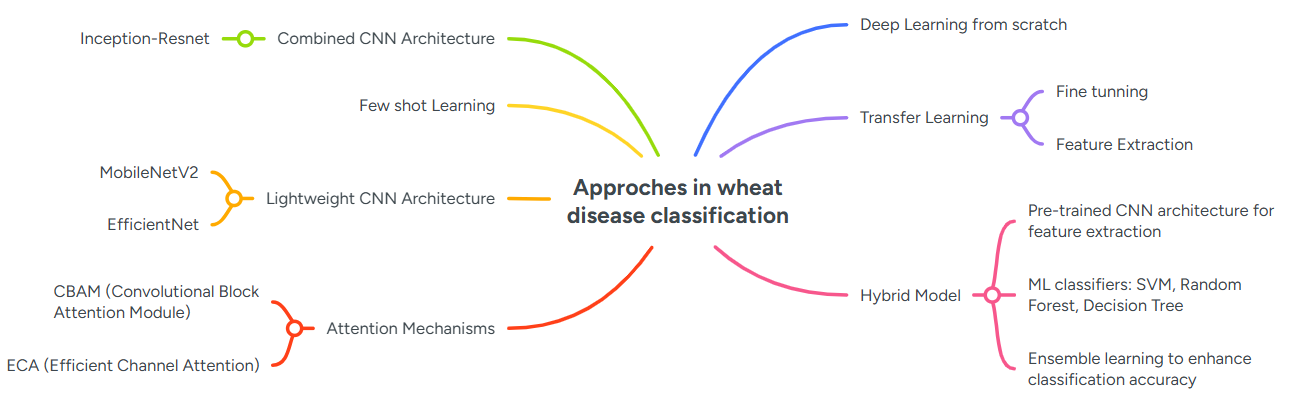
\includegraphics[width=0.8
    \textwidth]{chapters/chapter3/images/Figure01.png}
    \caption{Image acquisition techniques \protect\parencite{ghazal2024computer}.}
    \label{fig:ImageAcquisition}
\end{figure}



\subsection{RGB Cameras (Red, Green, Blue)}
RGB cameras are the most common type of imaging technology used in remote sensing. They capture images in the visible light spectrum (red, green, and blue wavelengths), similar to how the human eye perceives the world \parencite{delavarpour2021technical}. As shown in Figure~\ref{fig:RGBbackground}, RGB imagery can also be processed to remove non-vegetative elements such as soil background, enhancing the visibility of plant features \parencite{li2024monitoring}.

\begin{figure}[H]
    \centering
    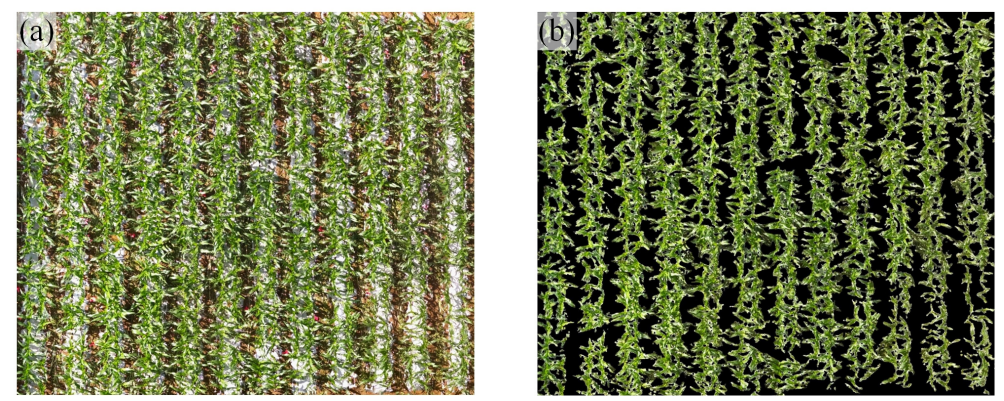
\includegraphics[width=0.6
    \textwidth]{chapters/chapter3/images/Figure02.png}
    \caption{RGB original image (a) and RGB image after removal of soil background (b) \protect\parencite{li2024monitoring}.}
    \label{fig:RGBbackground}
\end{figure}

\subsection{Near-Infrared (NIR) Cameras}

Near-infrared (NIR) cameras capture images in the near-infrared spectrum, which lies just beyond the visible light range. These cameras are sensitive to light wavelengths that are not visible to the human eye, typically ranging from 700 to 1300 nm \parencite{delavarpour2021technical}. NIR imaging is particularly valuable in plant health monitoring as it can detect subtle changes in vegetation that are not visible in the visible light spectrum. Figure~\ref{fig:UAVsensors} shows an example of a UAV equipped with NIR sensors used for such applications.


\begin{figure}[H]
    \centering
    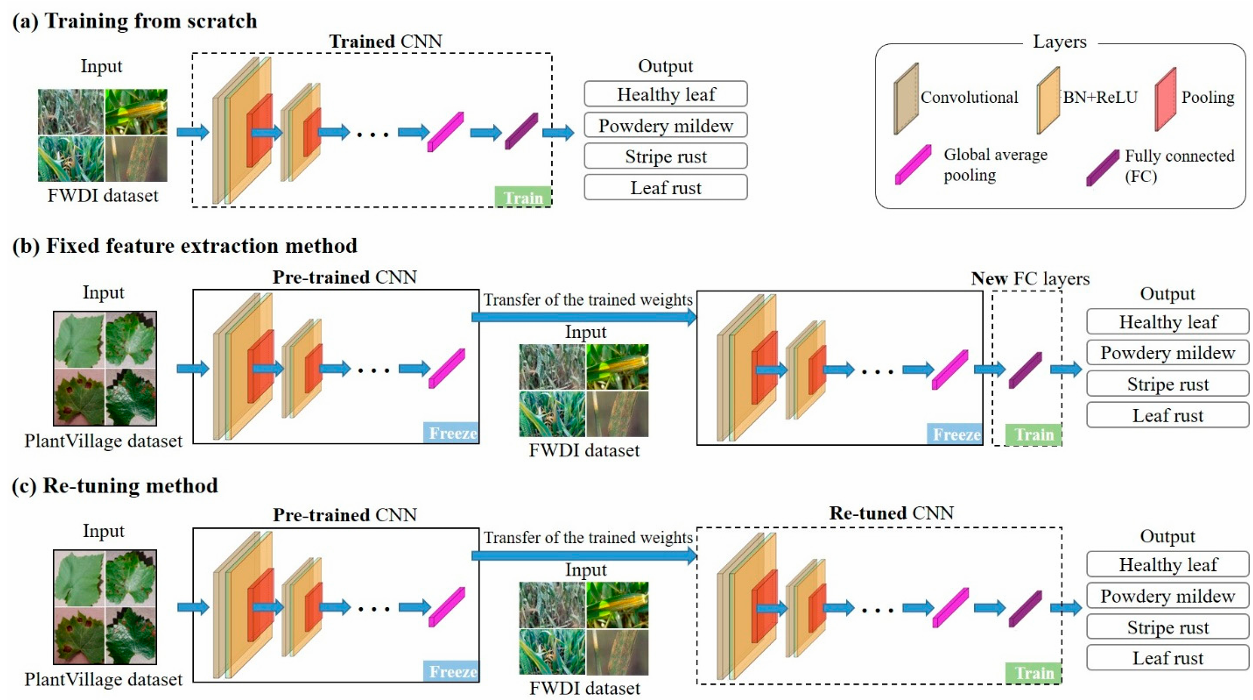
\includegraphics[width=0.6
    \textwidth]{chapters/chapter3/images/Figure03.png}
    \caption{The UAV and its sensors \protect\parencite{li2024monitoring}.}
    \label{fig:UAVsensors}
\end{figure}


\subsection{Thermal Infrared Cameras}

Thermal infrared cameras capture images based on the heat emitted by objects, operating in the infrared spectrum (wavelengths typically ranging from 8,000 to 14,000 nm). They detect temperature differences and translate them into visual representations, making them invaluable for identifying heat-related patterns in crops and soil \parencite{delavarpour2021technical}. This capability is demonstrated in Figure~\ref{fig:thermalimages}, which shows thermal and RGB images captured at different UAV flight heights.


\begin{figure}[H]
    \centering
    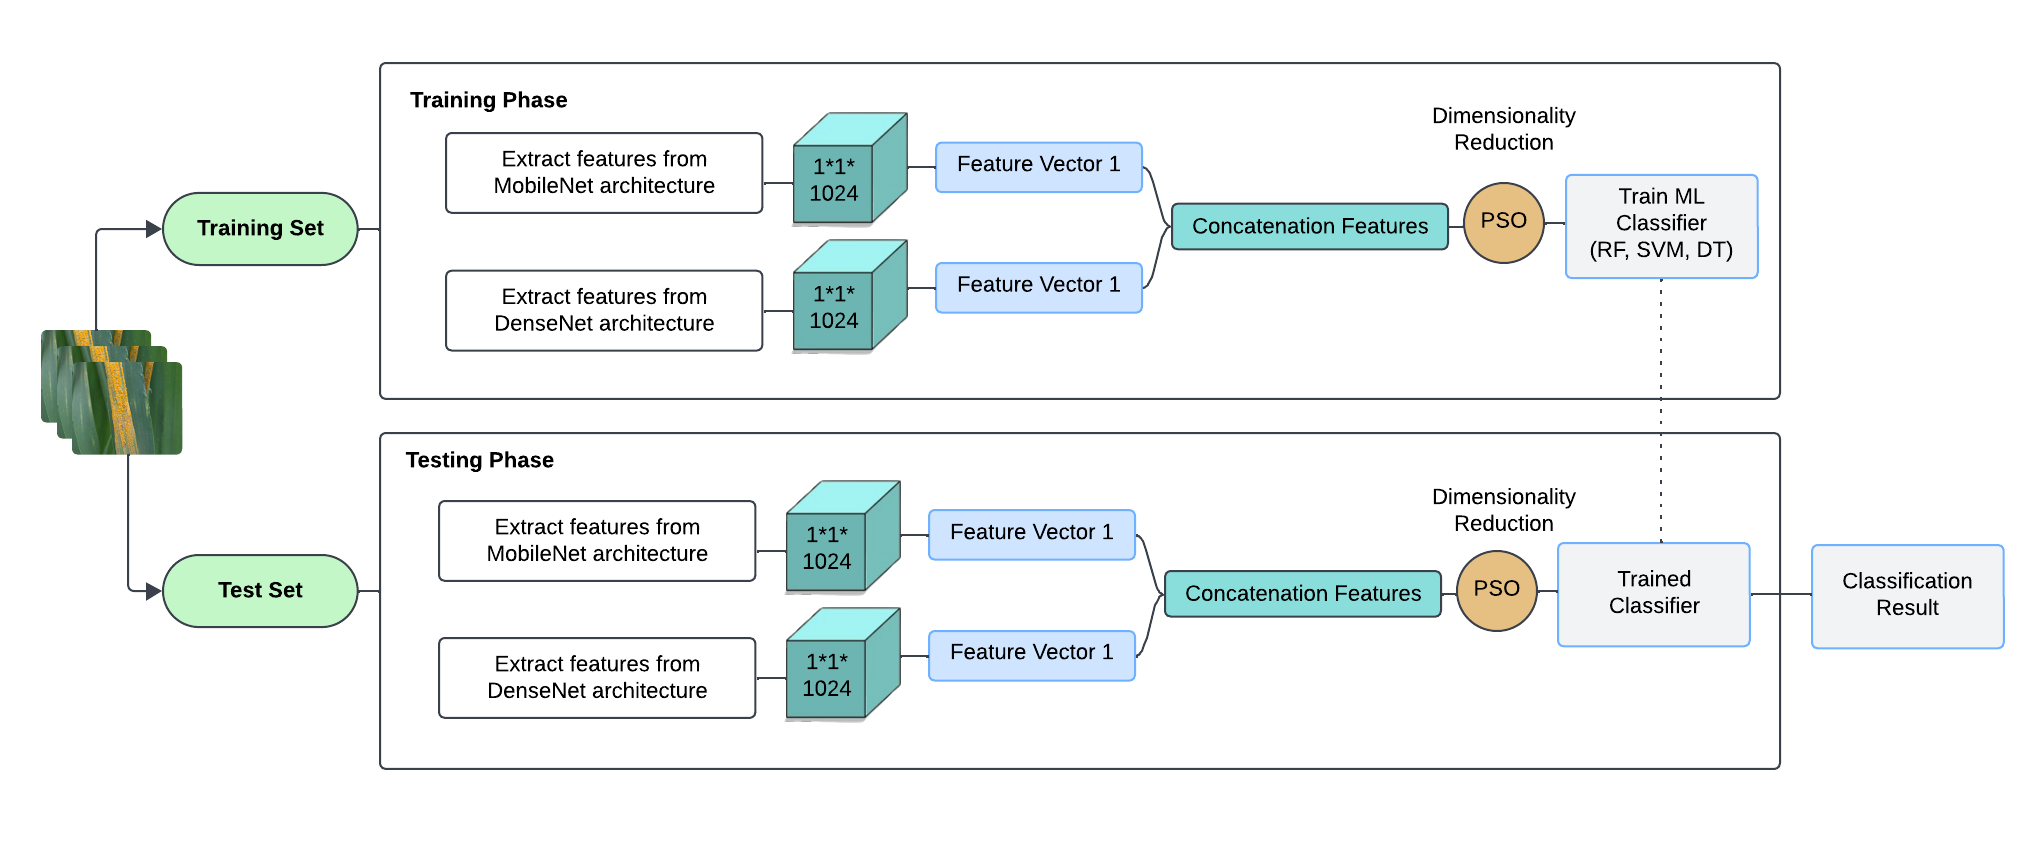
\includegraphics[width=0.8
    \textwidth]{chapters/chapter3/images/Figure04.png}
    \caption{Examples of acquired thermal images from FLIR Tau 2 and WIRIS 2nd Gen at two different UAV flight heights. RGB images acquired by the RGB cameras mounted on the same UAVs were also provided. ‘‘T’’ in the graphs refers to the measured temperature by the corresponding thermal cameras \protect\parencite{wan2024optimizing}.}
    \label{fig:thermalimages}
\end{figure}


\subsection{Multispectral Cameras}

Multispectral cameras capture images across multiple spectral bands, including visible (red, green, blue) and non-visible wavelengths (near-infrared and red-edge) across a limited number of discrete bands, each covering a wider spectral range spanning tens to hundreds of nanometers \parencite{lu2020recent}. These cameras typically have 5 to 10 bands, enabling detailed analysis of plant health and environmental conditions \parencite{delavarpour2021technical}. They are essential for applications that require data beyond what RGB cameras can provide.

\subsection{LiDAR Cameras (Light Detection and Ranging)}

LiDAR cameras use laser pulses to measure distances by calculating the time it takes for the laser to bounce back from a surface. This technology generates high-resolution 3D maps, capturing detailed information about the shape and structure of the terrain, vegetation, and other objects. LiDAR operates effectively in various environmental conditions, including low light or dense canopy cover \parencite{delavarpour2021technical}.

\subsection{Hyperspectral Cameras}
Hyperspectral cameras capture images across a vast range of continuous, narrow spectral bands, often exceeding hundreds. These bands typically have a spectral resolution below 10 nanometers, covering both visible and non-visible wavelengths. The fine-scale spectral data collected allows for the detection of subtle variations in reflectance, enabling detailed analysis of crop conditions, such as disease identification and nutrient stress. This high-resolution imaging is crucial for precision agriculture, where detecting subtle differences can significantly impact decision-making and yield optimization \parencite{delavarpour2021technical} \parencite{lu2020recent}.

\section{Remote Sensing Platforms}
Remote sensing platforms are categorized based on their altitude and mobility, each offering unique capabilities for capturing agricultural data. The three main types are satellite-based imaging, UAV (drone) imaging, and aircraft imaging.

\subsection{Satellite-Based Imaging}
Satellite-based imaging involves the use of Earth-observing satellites equipped with multispectral sensors to capture detailed images of the Earth's surface. These satellites, such as Quickbird and Landsat-1, can capture high-resolution images, providing data with varying levels of precision. Early satellite systems offered up to 6.5 meters per pixel in resolution \parencite{phang2023satellite}, while modern systems have significantly improved both spatial and spectral resolution. These advancements enable more accurate and comprehensive monitoring of large areas, laying the foundation for a wide range of applications, including agriculture and environmental studies \parencite{adao2017hyperspectral}. Despite its many advantages, satellite-based imaging also presents several challenges and limitations that must be considered in agricultural applications, including:

\begin{itemize}
    \item \textbf{Coarse Resolution:} The resolution of satellite imagery can be too coarse for some applications. For instance, imagery from platforms like Sentinel-2 (up to 10 m resolution) may not be detailed enough for fields with closely spaced rows, such as vines, leading to mixed pixel data that combines multiple rows and soil \parencite{adao2017hyperspectral}.
    
    \item \textbf{Data Processing Complexity:} Due to the coarse resolution, advanced methods like computer vision classifiers and statistical decision trees are often required to extract useful information, such as detecting shrubs or distinguishing plant species \parencite{phang2023from}.
    
    \item \textbf{Mixed Pixel Issue:} Low-resolution pixels, like those from Landsat, result in mixed data, complicating analysis and interpretation, especially in detailed applications \parencite{delavarpour2021technical}.
    
    \item \textbf{Spatiotemporal Challenges:} Obtaining timely spatiotemporal data on crop phenological status during critical growth periods is difficult, especially due to cloud coverage \parencite{delavarpour2021technical}.
    
    \item \textbf{High Costs:} Accessing satellite data equipped with multispectral sensors can be expensive, which limits its use for some applications \parencite{delavarpour2021technical}.
  \end{itemize}
  

\subsection{Aircraft-Based Imaging}

Aircraft-based imaging involves the use of piloted or unpiloted aircraft, such as airplanes, equipped with various remote sensing tools to capture high-resolution imagery and sensor data over large agricultural areas. These systems offer a significant advantage in large-scale applications due to their flexibility and ability to carry heavier payloads of sensors, making them a viable alternative to satellite-based or UAV-based solutions \parencite{delavarpour2021technical}.
Before the widespread adoption of UAVs, manned aircraft were commonly employed for lower-to-ground remote sensing, utilizing multi-spectral or electro-optic (EO) sensors to monitor agricultural conditions \parencite{phang2023satellite}, However, this approach also faces several limitations, including:

\begin{itemize}
    \item \textbf{High Operational Costs:} Operating aircraft-based systems involves significant expenses for fuel, maintenance, and pilot salaries, making them less affordable compared to UAVs \parencite{delavarpour2021technical, phang2023from}.
    
    \item \textbf{Complex Logistics and Pilot Requirement:} Certified pilots and specific flight logistics are essential, adding complexity and reducing flexibility in deployment \parencite{adao2017hyperspectral}.
    
    \item \textbf{Limited Flexibility:} Aircraft require designated takeoff and landing zones, restricting their use in remote or uneven terrains \parencite{delavarpour2021technical}.
    
    \item \textbf{Weather Sensitivity:} Adverse weather conditions, such as strong winds or rain, can impact flight stability and data quality, limiting operations during critical periods \parencite{delavarpour2021technical}.
    
    \item \textbf{Regulatory and Airspace Restrictions:} Aircraft-based systems are subject to strict aviation regulations and airspace restrictions, limiting their operational scope \parencite{delavarpour2021technical}.
    
    \item \textbf{High Data Processing Requirements:} Large volumes of data generated require specialized software and computing resources, making data processing resource-intensive \parencite{delavarpour2021technical}.
    
    \item \textbf{Costly for Large-Scale Use:} The expense and complexity of these systems make them impractical for frequent large-scale monitoring, favoring UAV alternatives for cost efficiency \parencite{phang2023from}.
    
    \item \textbf{Resolution Limitations:} Although aircraft provide better resolution than satellites, their imagery can still be too coarse for some precision applications \parencite{adao2017hyperspectral}.
  \end{itemize}
  
\subsection{UAV-Based Imaging}

Unmanned Aerial Vehicles (UAVs), or drones, are versatile remote sensing platforms that have become essential tools in remote sensing due to their cost-effectiveness, flexibility, and ability to capture high-resolution (cm-level) images, making them ideal for precision agriculture \parencite{sishodia2020applications}. UAV-based imaging typically involves using low-altitude remote Sensing Systems (LARS) to acquire detailed imagery of the Earth’s surface at low altitudes, providing high precision and adaptability \parencite{phang2023satellite}.

Unlike traditional satellite platforms, UAVs offer several advantages, including on-demand data collection, high-resolution imagery, and flexible deployment, which enable real-time monitoring and analysis \parencite{phang2023satellite}. A complete Unmanned Aerial System (UAS) includes the UAV and its remote sensing equipment, operating without a human pilot onboard, and is capable of carrying various sensors tailored to different agricultural needs \parencite{adao2017hyperspectral}, Despite their advantages, UAVs also face some challenges, including:

\begin{itemize}
    \item \textbf{Short Flight Duration:} UAVs, especially smaller models, often have flight durations of less than 30 minutes, which limits their coverage area, particularly for large-scale agricultural operations \parencite{phang2023from}.
    
    \item \textbf{Regulatory Challenges:} Stricter regulations, especially for larger UAVs, slow down their adoption and innovation, hindering their widespread use \parencite{phang2023from, delavarpour2021technical}.
    
    \item \textbf{Scalability:} UAV-based remote sensing requires trained pilots and continuous monitoring, which limits scalability, particularly for small-scale applications \parencite{phang2023from}.
    
    \item \textbf{Environmental Sensitivity and Calibration Issues:} Hyperspectral sensors on UAVs face challenges related to environmental factors such as light exposure and atmospheric interference, necessitating frequent recalibration \parencite{adao2017hyperspectral}.
    
    \item \textbf{Weather Dependency:} UAVs are susceptible to weather conditions like wind and rain, which can affect both flight stability and data quality \parencite{delavarpour2021technical}.
    
    \item \textbf{Battery Life:} The limited battery life of UAVs impacts their ability to cover large areas, particularly in extensive agricultural fields \parencite{delavarpour2021technical}.
  \end{itemize}
  
\section{Vegetation Indices}
Vegetation indices are mathematical formulas that combine light reflectance data from different spectral bands (such as visible, near-infrared, and mid-infrared) captured by sensors on drones or satellites to assess plant health and condition. These indices provide valuable insights into growth stages, plant vigor, biomass, and chlorophyll levels \parencite{sishodia2020applications}. Plants reflect sunlight differently based on their type, structure, and water content: they reflect little in the blue and red regions, more in green (which makes them appear green), and strongly in the near-infrared (NIR) if healthy (Figure~\ref{fig:bluegreenred}). 

\begin{figure}[H]
    \centering
    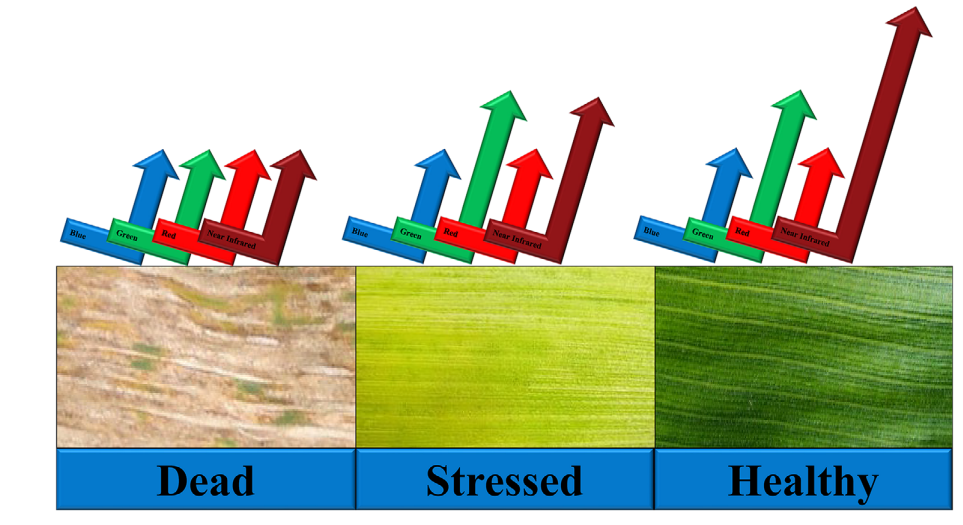
\includegraphics[width=0.8
    \textwidth]{chapters/chapter3/images/Figure05.png}
    \caption{Unique optical reflectance signature differences of blue, green, red, and near-infrared light emitted from dead, stressed, and healthy plant tissue \protect\parencite{olson2021review}.}
    \label{fig:bluegreenred}
\end{figure}


Thermal and infrared indices, including CWSI (Crop Water Stress Index) and SIWSI (Shortwave Infrared Water Stress Index), use thermal radiation data to estimate plant temperature, water stress, and transpiration, aiding in drought detection, crop yield estimation, and disease monitoring \parencite{sishodia2020applications}. For more vegetation indices, their mathematical formulas, and detailed applications, refer to Appendix~\ref{app:annexA}.
\begin{table}[htbp]
    \caption{Some recently used vegetation indices for remote sensing applications in precision agriculture.}
    \centering
    \resizebox{\textwidth}{!}{%
    \begin{tabular}{|p{4cm}|p{5cm}|p{6cm}|}
    \hline
    \textbf{Spectral Index} & \textbf{Equation} & \textbf{Application} \\
    \hline
    Normalized Difference Vegetation Index (NDVI) & $NDVI = \frac{\text{NIR} - \text{Red}}{\text{NIR} + \text{Red}}$ & Measure of healthy, green vegetation \\
    \hline
    Green Normalized Difference Vegetation Index (GNDVI) & $GNDVI = \frac{\text{NIR} - \text{Green}}{\text{NIR} + \text{Green}}$ & Measure of healthy, green vegetation; higher chlorophyll concentration sensitivity than NDVI \\
    \hline
    Red Edge Normalized Difference Vegetation Index (RENDVI) & $RENDVI = \frac{\text{NIR} - \text{Red Edge}}{\text{NIR} + \text{Red Edge}}$ & Modification of NDVI; capitalizes on the sensitivity of the vegetation red edge \\
    \hline
    Soil Adjusted Vegetation Index (SAVI) & $SAVI = \frac{1.5(\text{NIR} - \text{Red})}{\text{NIR} + \text{Red} + 0.5}$ & Modification of NDVI; suppresses the effects of soil pixels \\
    \hline
    Atmospherically Resistant Vegetation Index (ARVI) & $ARVI = \frac{\text{NIR} - (\text{Red} - \text{Blue})}{\text{NIR} + (\text{Red} - \text{Blue})}$ & Disease; weed mapping \\
    \hline
    Wide Dynamic Range Vegetation Index (WDRVI) & $WDRVI = \frac{\text{NIR} - \text{Red}}{\text{NIR} + \text{Red}}$ & N-Application, yield; crop growth (LAI); disease \\
    \hline
    Normalized Difference Red Edge (NDRE) & $NDRE = \frac{\text{NIR} - \text{Red Edge}}{\text{NIR} + \text{Red Edge}}$ & Crop yield and biomass; N-management; disease \\
    \hline
    Red Edge DVI (REDVI) & $REDVI = \text{NIR} - \text{Red Edge}$ & Crop yield and biomass; biomass, N-uptake, and concentration \\
    \hline
    \end{tabular}%
    }
    \label{tab:vegetation-indices}
\end{table}





\section{Image processing}

Imagery processing is the technique used to turn multiple aerial images captured by drones (UAVs) or remote sensors into a single, accurate, and clear image known as an orthomosaic. Since drones don’t capture one large image but instead take many smaller ones of different parts of the area, these images must be merged using a process called image stitching  (as shown in Figure~\ref{fig:UAVDataProducts}), This involves merging individual images into one large composite by identifying and aligning “key points” such as a rock, plant, or edge of a field. While the drone captures these images, it simultaneously records GPS or location metadata, which is then used in geographic alignment to position each image on a map accurately. The final output of this process is known as data products, which can include color mosaics (stitched colored images), spectral mosaics (capturing invisible wavelengths like near-infrared for agricultural analysis), thermal mosaics (highlighting temperature variations), surface and terrain models (representing elevation and landscape shapes), and point clouds (dense 3D representations of surfaces for detailed analysis) \parencite{olson2021review}.

\begin{figure}[H]
    \centering
    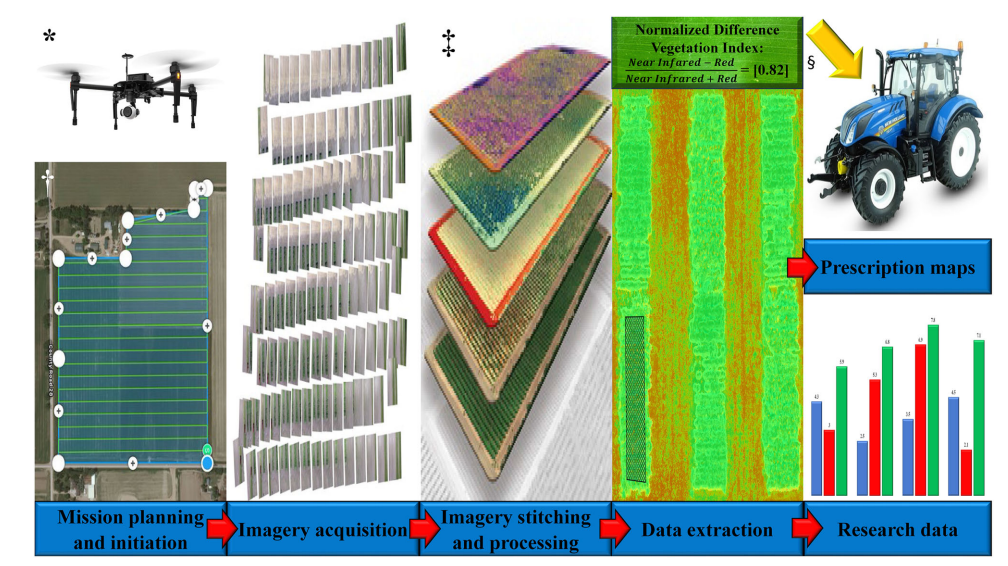
\includegraphics[width=0.8
    \textwidth]{chapters/chapter3/images/Figure06.png}
    \caption{Standard Workflow for Generating UAV-Derived Imagery and Data Products \protect\parencite{olson2021review}.}
    \label{fig:UAVDataProducts}
\end{figure}

Imagery can be processed on-site with personal computers and the appropriate software or in the field with cloud computing imagery processing \parencite{olson2021review}. The pros and cons of each imagery processing option are discussed in Table~\ref{tab:ProcessingMethodComparison}.

\begin{table}[h]
    \centering
    \renewcommand{\arraystretch}{1.5} % Increase row height
    \setlength{\tabcolsep}{8pt} % Adjust column padding
    \begin{tabular}{|p{3cm}|p{5.5cm}|p{5.5cm}|}
    \hline
     & \textbf{Pros} & \textbf{Cons} \\ \hline
    
     \multirow{4}{*}{\parbox{2.8cm}{\centering\textbf{Software (On-Site Processing on PC)}}}    & Customizable options & High-performance PC needed \\ \cline{2-3}
    & No limits on images & Expensive initial cost \\ \cline{2-3}
    & GIS software compatible & Steep learning curve \\ \cline{2-3}
    & One-time purchase & Slower processing \\ \hline
    
    \multirow{4}{*}{\parbox{2.8cm}{\centering\textbf{Cloud Computing (Online/Remote Processing)}}}    & Easy to use & Fewer customizations \\ \cline{2-3}
    & Low upfront cost & Image limits \\ \cline{2-3}
    & Fast field processing & Ongoing costs \\ \cline{2-3}
    & No powerful PC needed & \\ \cline{2-3}
    & Simplified analysis & \\ \hline
    \end{tabular}
    \caption{Comparison of On-Site Software vs. Cloud Computing for Imagery Processing \parencite{olson2021review}.}
    \label{tab:ProcessingMethodComparison}
    \end{table}
    

\section{Applications of Remote Sensing Data}
Remote sensing has diverse applications in agriculture, enabling precise, data-driven decision-making. It helps monitor field conditions, optimize resource use, and address issues early. The following sections highlight key areas where remote sensing enhances farm management:

\begin{itemize}[leftmargin=1.5em]

    \item \textbf{Crop Health Monitoring:} Remote sensing enables regular monitoring of crop conditions, helping detect diseases, pest presence, and water or nutrient stress early. Vegetation indices (e.g., NDVI) derived from RGB, NIR, multi-spectral, and hyperspectral sensors are commonly used to assess aspects such as foliage cover, pigment composition, and water stress. LiDAR and GPS can also support the accurate mapping of plant structure and spatial positioning. These technologies collectively support better crop management and yield optimization \parencite{phang2023satellite}.
    
    \item \textbf{Weed Control:} Precise weed detection helps reduce competition for water, nutrients, and light. Aerial imagery from UAVs and satellite platforms, often using RGB and multispectral cameras, supports vegetation indexing and mapping for weed identification. Some systems enable real-time onboard image analysis and spraying. These tools assist in implementing targeted and efficient weed management strategies while reducing input costs \parencite{phang2023satellite}.
    
    \item \textbf{Infectious Disease Epidemiology and Mapping:} UAVs are used to gather high-resolution spatial data for studying the relationships between environmental conditions and disease spread. They help monitor changes in land use, population distribution, and vegetation patterns, which are valuable for identifying and mitigating disease risks affecting crops or livestock. UAV-collected data provide flexible, cost-effective alternatives to satellite and manned aerial surveys \parencite{phang2023satellite}.
    
    \item \textbf{Spectral Imaging:} Multispectral and hyperspectral imaging technologies offer detailed insights into crop nutrient levels, stress, and overall vigor. Though hyperspectral data offer higher spectral resolution, they also require more complex processing, often conducted post-flight. These systems rely on sensors like CCD and CMOS and use scanning methods such as point, line, and plane scanning. Accurate georeferencing is achieved using ground control points (GCPs) or advanced navigation systems \parencite{phang2023satellite}.
    
\end{itemize}

\section{Workflow for Integrating Remote Sensing and ML/DL in Wheat Disease Detection}
Existing research on crop disease detection using UAV imagery can be grouped into three main methodological approaches (Figure~\ref{fig:Classificationapproaches}). The first involves statistics-based methods, which apply correlation and regression analyses to identify linear relationships between disease symptoms and spectral data from UAV images. These methods commonly use vegetation indices (VIs) to extract relevant crop traits. The second approach includes conventional machine learning techniques, where VIs serve as input features for supervised or unsupervised models used in disease estimation. The third and most recent approach is based on deep learning, which leverages raw UAV images alongside other features to train end-to-end models for automated crop disease recognition \parencite{shahi2023recent}.


\begin{figure}[H]
    \centering
    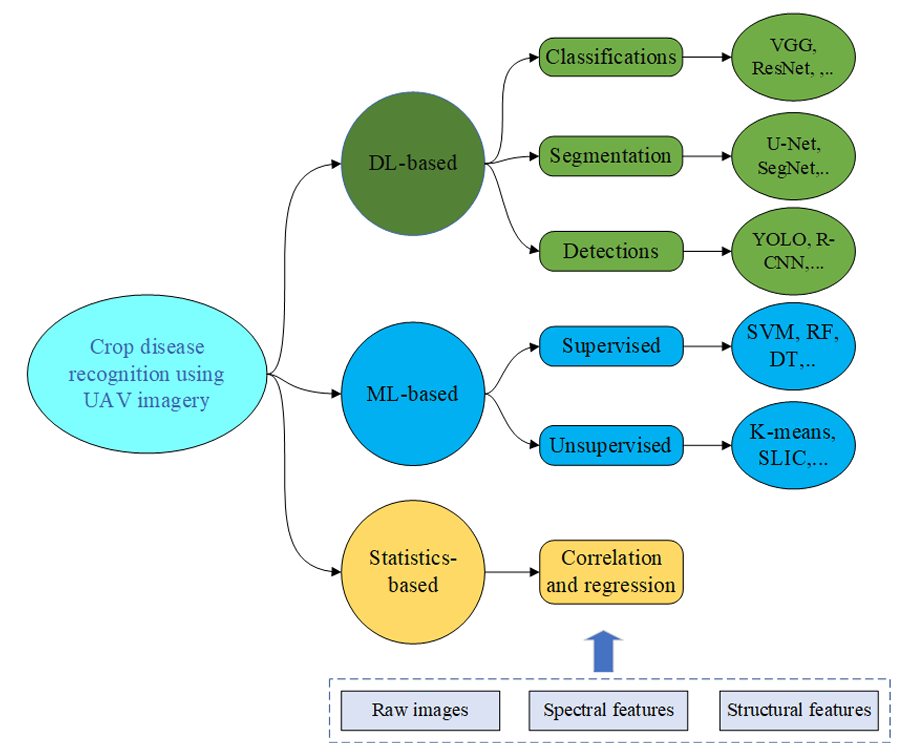
\includegraphics[width=0.8
    \textwidth]{chapters/chapter3/images/Figure07.png}
    \caption{Classification of crop disease detection approaches using UAV-based remote sensing. The elements within the dotted box represent the image features utilized across one or more of the listed approaches \parencite{shahi2023recent}.}
    \label{fig:Classificationapproaches}
\end{figure}

\subsection{Features Extraction}
In the context of remote sensing for plant disease detection, different types of features can be extracted from imagery to capture various physiological, structural, and visual properties of crops.

\begin{itemize}
    \item \textbf{Spectral Features}: Describe how plants reflect light across different spectral bands (such as visible, red edge, or near-infrared). These features reveal the biochemical state of vegetation, helping detect conditions like chlorophyll content, moisture level, and early stress symptoms using vegetation indices (e.g., NDVI, NDRE) or raw spectral band reflectance \parencite{Dhakal2023spectral}.
    
    \item \textbf{Structural Features}: Represent the physical shape, size, and arrangement of plant components, such as canopy height, leaf area, or plant density. They help monitor growth patterns and identify visible deformations caused by disease, pests, or environmental stress through 3D models or spatial measurements \parencite{Dhakal2023spectral}.
    
    \item \textbf{Textural Features (TF)}: Capture the variation and arrangement of pixel intensities in an image, describing surface patterns like roughness, smoothness, or regularity. These features are useful for detecting visual symptoms of disease, such as lesions or uneven leaf surfaces, using statistical metrics like contrast, entropy, and homogeneity \parencite{Dhakal2023spectral}.
    
    \item \textbf{Wavelet Features (WF)}: Capture spatial and spectral variations in data by breaking it down into components at different scales. These features can detect fine-scale patterns, which are useful for identifying subtle changes in vegetation, such as variations caused by disease or stress \parencite{Ma2021FusariumUAV}.
 
\end{itemize}
  

\subsection{Statistics-Based Methods}
Statistics-based methods for crop disease estimation rely on using crop-related traits derived from UAV imagery as independent variables and disease scores as the target variable. These methods typically involve three main steps: image pre-processing, vegetation index (VI) generation, and statistical analysis. During pre-processing, spatial data products such as reflectance maps are generated, representing how much light vegetation reflects across different wavelengths, which is crucial for assessing plant health. These maps calculate various vegetation indices (e.g., NDRE, NDVI, and DVI) to summarize plant conditions like chlorophyll content, stress, or canopy vigor. These indices are then used in correlation and regression analyses to estimate disease severity \parencite{shahi2023recent}.

In practice, fields are often divided into small plots, and the mean VI value per plot is computed for analysis. Some studies also apply threshold-based techniques, setting a cutoff value to distinguish between healthy and diseased areas. However, defining a universal threshold is difficult due to variability in crop type, disease symptoms, and imaging conditions.

For example, \parencite{guo2021wheat} employed UAV-based hyperspectral imagery to detect wheat yellow rust and incorporated both vegetation indices (VIs) and texture features (TFs) into their statistical models. \parencite{guo2021wheat} extracted TFs using Principal Component Analysis (PCA), followed by methods like the Gray-Level Co-occurrence Matrix (GLCM), a technique used to analyze the spatial relationship between pixel intensities in an image. GLCM captures texture features such as contrast, entropy, and correlation, which help detect subtle patterns in plant surfaces that could indicate disease or stress. By combining these TFs with spectral indices in a Partial Least Squares Regression (PLSR) model, they achieved significantly higher accuracy, reaching an \( R^2 \) of 0.88 in the late infection stage.
PLSR is a regression technique that is particularly effective when the predictors are many and possibly collinear, as it reduces dimensionality and finds the most relevant directions for predicting the response variable. The general form of the PLSR equation~\eqref{eq:plsr} is:

\begin{equation}
Y = \beta_0 + \beta_1X_1 + \beta_2X_2 + \ldots + \beta_nX_n
\label{eq:plsr}
\end{equation}

where $Y$ is the disease severity index, $X_1, \ldots, X_n$ are the input features (e.g., VIs, TFs), and $\beta_0, \ldots, \beta_n$ are the regression coefficients determined during model training.

Their study also highlighted that high spatial resolution (10–15 cm) images were critical for capturing fine structural differences caused by disease. Similarly, \parencite{bhandari2020assessing} achieved a strong correlation ($R^2 = 0.79$) using the GLI index derived from RGB images to assess foliar diseases in wheat (Table~03). Together, these studies show that combining spectral and textural information enhances the performance of statistical models in UAV-based crop disease monitoring.

The detailed formulas for the vegetation indices (VIs) used in the studies mentioned are provided in Appendix~\ref{app:annexA}.
\begin{table}[htbp]
    \caption{Summary of ST-based methods for Wheat disease estimation using UAV imagery.}
    \centering
    \resizebox{\textwidth}{!}{%
    \begin{tabular}{|p{3.5cm}|p{3.5cm}|p{3cm}|p{4cm}|p{3cm}|}
    \hline
    \textbf{Paper} & \textbf{Disease} & \textbf{Sensor} & \textbf{Vegetation Indices (VIs)} & \textbf{Eval. Metrics} \\
    \hline
    \parencite{bhandari2020assessing} & Wheat foliage disease & RGB & NDI, GI, GLI & $R^2 = 0.79$ \\
    \hline
    \parencite{HeidarianDehkordi2020} & Leaf rust, Stem rust & RGB & SRI, LRI & $R^2 = 0.81$ \\
    \hline
    \parencite{guo2021wheat} & Yellow rust & Hyperspectral & SIPI, PRI, TCARI, PSRI, YRIGI & $R^2 = 0.88$ \\
    \hline
    \parencite{Khan2021} & Powdery Mildew & Hyperspectral & PMI, MSR, MCARI & $R^2 = 0.722$ \\
    \hline
    \end{tabular}%
    }
    \label{tab:summary}
\end{table}



\subsection{Conventional Machine Learning (ML)-Based Methods}
Traditional machine learning (ML) methods, including support vector machines (SVMs), artificial neural networks (ANNs), Support Vector Regression (SVR), have been applied to crop disease detection using UAV imagery. These methods aim to identify patterns in labeled or unlabeled data, with supervised learning relying on labeled datasets for training and unsupervised learning exploring hidden patterns without labels \parencite{shahi2023recent}. The typical ML pipeline involves data collection, preprocessing, feature extraction, and model building, as shown in Figure~\ref{fig:MLBased}.

\begin{figure}[H]
    \centering
    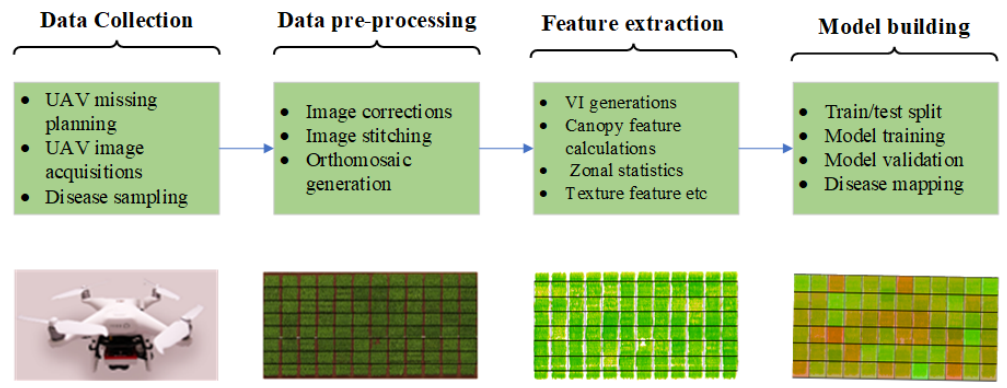
\includegraphics[width=0.8
    \textwidth]{chapters/chapter3/images/Figure08.png}
    \caption{General Workflow of Conventional ML-Based Crop Disease Detection Using UAV Imagery \parencite{shahi2023recent}.}
    \label{fig:MLBased}
\end{figure}


Researchers have applied various machine learning (ML) methods to detect wheat diseases, with different results depending on the disease type and the input features used. Here is a detailed explanation of the studies:

\begin{itemize}
    \item \textbf{\parencite{liu2020monitoring}}  worked on detecting Fusarium head blight using hyperspectral sensors. They utilized spectral bands, vegetation indices, and texture features as input features. They applied a Backpropagation neural network with Simulated Annealing, a technique that helps optimize the model by avoiding local minima, and achieved a high accuracy of 98\%.
    \item \textbf{\parencite{Ma2021FusariumUAV}} focused on detecting Fusarium head blight using hyperspectral sensors. They used spectral bands, vegetation indices, and wavelet features. The machine learning method employed was Support Vector Machine (SVM), which yielded a coefficient of determination (R²) of 0.88, indicating a strong predictive performance.
    \item \textbf{\parencite{zhu2022using}} worked on detecting wheat scab using multispectral sensors. They used vegetation indices and texture features as input features. The models used for analysis included Partial Least Squares Regression (PLSR), Support Vector Regression (SVR), and Backpropagation Neural Networks (BPNN), achieving an R² value of 0.83.
    \item \textbf{\parencite{bohnenkamp2019in}} focused on detecting yellow rust using hyperspectral sensors, with vegetation indices as the primary input feature. They applied the Support Vector Machine (SVM) method and obtained an R² value of 0.63.
\end{itemize}

Table~\ref{tab:summaryML} provides a summary of conventional machine learning methods for wheat disease estimation, highlighting the combination of sensor types, features, and machine learning techniques employed to improve disease detection accuracy.

\begin{table}[htbp]
    \caption{Summary of conventional ML methods for wheat disease estimation.}
    \centering
    \resizebox{\textwidth}{!}{%
    \begin{tabular}{|p{3.5cm}|p{3cm}|p{2cm}|p{4cm}|p{3cm}|p{2.5cm}|}
    \hline
    \textbf{Reference} & \textbf{Disease} & \textbf{Sensors} & \textbf{Features} & \textbf{ML Methods} & \textbf{Eval. Metrics} \\
    \hline
    \parencite{liu2020monitoring} & Fusarium head blight & HS & SBs (spectral bands), VI, TF (texture features) & BP with SA & Accuracy = 0.98 \\
    \hline
    \parencite{Ma2021FusariumUAV} & Fusarium head blight & HS & SBs (spectral bands), VIs, WFs & SVM & $R^2 = 0.88$ \\
    \hline
    \parencite{zhu2022using} & Wheat scab & MS & VI, TF (texture features) & PLSR, SVR, BPNN & $R^2 = 0.83$ \\
    \hline
    \parencite{bohnenkamp2019in} & Yellow rust & HS & VIs & SVM & $R^2 = 0.63$ \\
    \hline
    \end{tabular}%
    }
    \label{tab:summaryML}
\end{table}


\subsection{Deep Learning (DL)-Based Methods}

Deep learning methods have been widely applied for crop disease estimation using UAV imagery. The general pipeline for deep learning-based crop disease detection is shown in Figure~\ref{fig:DLBased} and includes data collection, preparation, model building, and evaluation. However, specific tasks such as image stitching, tiling, and annotation are critical during data preparation for UAV images. Deep learning models for crop disease detection can be categorized into classification-based, segmentation-based, and detection-based approaches. Segmentation models classify individual pixels as healthy or diseased, while classification models classify entire images into disease categories \parencite{shahi2023recent}. Detection-based models localize and label the area of interest within the image, as illustrated in Figure~\ref{fig:DLBased}.

\begin{figure}[H]
    \centering
    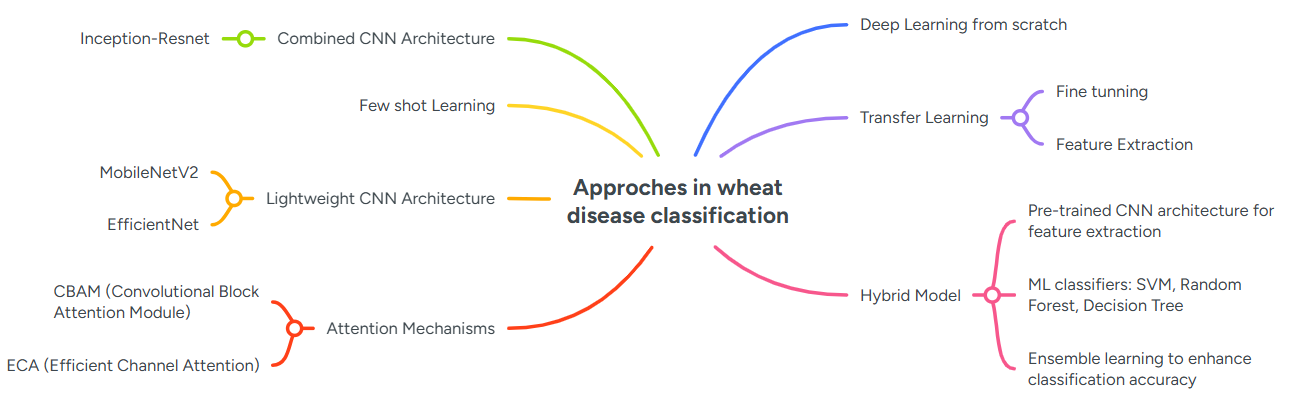
\includegraphics[width=0.8
    \textwidth]{chapters/chapter3/images/Figure09.png}
    \caption{General Workflow of DL-based crop disease detection using UAV imagery \parencite{shahi2023recent}.}
    \label{fig:DLBased}
\end{figure}

\subsubsection{Pixel-Based Segmentation Models}

Pixel-based segmentation models focus on classifying each pixel in an image based on its characteristics, allowing for precise detection of disease symptoms in specific areas of a plant or field. By analyzing the image at a granular level, these models assign labels to each pixel, helping to identify localized disease patterns across the crop. Several studies have applied such models to detect wheat diseases, yielding impressive results. For instance, \parencite{pan2021deep} used RGB sensors and the PSPNet model to detect yellow rust, achieving an accuracy of 94\%. Similarly, \parencite{su2020aerial} applied multispectral sensors and the U-Net model for yellow rust, achieving a recall of 0.926 and an F-score of 0.92. \parencite{deng2022applying} employed RGB sensors with the DeepLabv3+ model for stem rust, obtaining an F-score of 0.81. \parencite{zhang2021irunet} used RGB sensors and the lr-UNet model for yellow rust, achieving an accuracy of 97.13\%, while \parencite{zhang2022wheat} applied multispectral sensors with the UNet and DF-UNet models for yellow rust, achieving an accuracy of 96.93\%. These studies demonstrate the effectiveness of pixel-based segmentation models in detecting wheat diseases with high precision.

\subsubsection{Object-Level Classification Models}

Object-level classification models treat the image as a whole, classifying entire regions or objects within an image rather than individual pixels. These models focus on detecting the overall presence of diseases at the object or plant level, which is useful for broader assessments of crop health. For instance, \parencite{zhang2019deep} used hyperspectral sensors and the Inception-ResNet model for detecting yellow rust, achieving an accuracy of 85\%. Similarly, \parencite{huang2019detection} applied RGB sensors and a convolutional neural network (CNN) to detect Helminthosporium leaf blotch, achieving an accuracy of 91.43\%. These studies highlight the application of object-level classification models in detecting crop diseases at a larger scale, emphasizing overall disease presence across plant regions.

A summary of deep learning-based methods for wheat disease estimation is presented in Table~\ref{tab:dl_summary}. Overall, these deep learning approaches show great potential for fine-grained and scalable wheat disease monitoring in precision agriculture.
\begin{table}[htbp]
    \caption{Summary of deep learning-based methods for wheat disease estimation.}
    \centering
    \resizebox{\textwidth}{!}{%
    \begin{tabular}{|p{2cm}|p{4cm}|p{2cm}|p{4cm}|p{3.5cm}|p{3cm}|}
    \hline
    \textbf{Reference} & \textbf{Disease} & \textbf{Sensors} & \textbf{Task} & \textbf{DL Methods} & \textbf{Results} \\
    \hline
    \parencite{pan2021deep} & Yellow Rust & RGB & Pixel-Based Segmentation Models & PSPNet & Acc = 0.94 \\
    \hline
    \parencite{su2020aerial} & Yellow Rust & MS & Pixel-Based Segmentation Models & U-Net & Recall = 0.926, F-Score = 0.92 \\
    \hline
    \parencite{deng2022applying} & Stem Rust & RGB & Pixel-Based Segmentation Models & DeepLabv3+ & F-Score = 0.81 \\
    \hline
    \parencite{zhang2021irunet} & Yellow Rust & RGB & Pixel-Based Segmentation Models & lr-UNet & Acc = 0.9713 \\
    \hline
    \parencite{zhang2022wheat} & Yellow Rust & MS & Pixel-Based Segmentation Models & UNet, DF-UNet & Acc = 96.93 \\
    \hline
    \parencite{zhang2019deep} & Yellow Rust & HS & Object-Level Classification Models & Inception-ResNet & Acc = 0.85 \\
    \hline
    \parencite{huang2019detection} & Helminthosporium leaf blotch & RGB & Object-Level Classification Models & CNN & Acc = 0.9143 \\
    \hline
    \end{tabular}%
    }
    \label{tab:dl_summary}
\end{table}

    









RGB sensors are predominantly paired with deep learning (DL) methods, while MS sensors are more frequently used with machine learning (ML) approaches. This distinction is closely tied to the spatial resolution requirements of DL models, which demand high-resolution images typically captured at lower altitudes using RGB sensors. In contrast, ML models are more tolerant of lower-resolution imagery, often obtained from higher flight altitudes. As illustrated in Figure 10, most DL-based studies used UAV images taken below 20 meters, whereas ML-based studies tended to operate UAVs above 30 meters. The limited use of hyperspectral sensors in both ML and DL methods is likely due to their high cost and the complexity of data processing. These trends underscore the growing preference for cost-effective, high-resolution UAV setups in DL-based crop disease estimation \parencite{shahi2023recent}.


\begin{figure}[H]
    \centering
    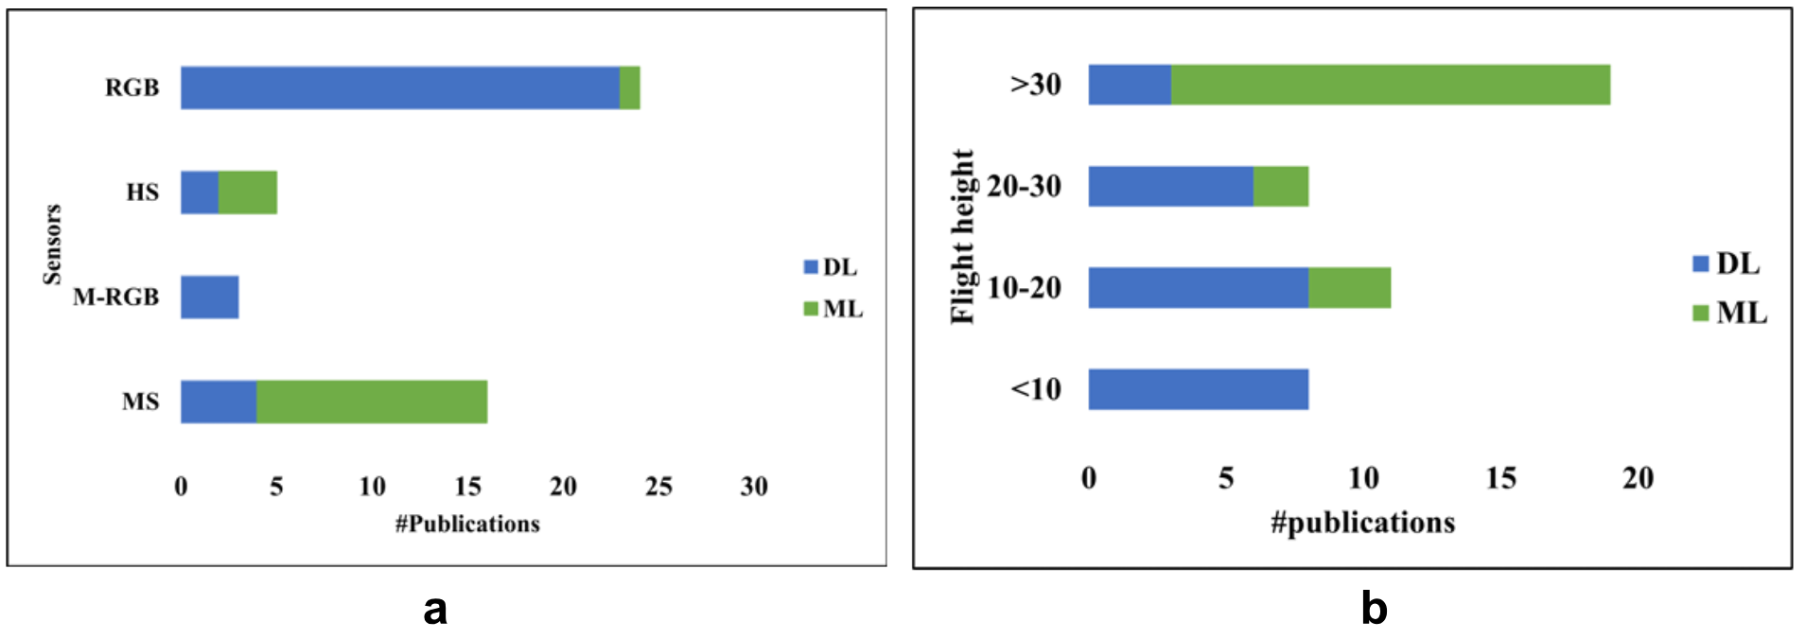
\includegraphics[width=0.8
    \textwidth]{chapters/chapter3/images/Figure10.png}
    \caption{The distribution of existing works based on (a) sensors and (b) flight altitudes used in UAV image acquisition. Note that M-RGB denotes modified RGB sensors \parencite{shahi2023recent}.}
    \label{fig:existingWorks}
\end{figure}


\section{Fusion of Satellite and UAV Data}

The fusion of satellite and UAV data presents a promising solution for overcoming the limitations of each platform in agricultural monitoring. While satellites offer broad and frequent coverage, their spatial resolution can be insufficient for detailed field assessments. UAVs provide high-resolution imagery but are limited in coverage and frequency. By combining these complementary strengths, it becomes possible to achieve accurate, timely, and scalable crop monitoring that supports more informed decision-making in precision agriculture \parencite{Maimaitijiang2020,Li2022}.

\subsection{Systematic Categorization of UAV/Satellite Monitoring Methods}
UAV/Satellite integration is categorized using a hierarchical decision tree based on three criteria (Figure~\ref{fig:UAVSatelliteStrategies}). The first distinguishes between weak and strong synergies: Weak synergy involves simple comparisons of UAV and satellite data, while strong synergy combines them to produce more informative outcomes. Among strong synergies, the second criterion differentiates between cases with the same observation target and those with different scales, known as “multiscale explanation,” where UAV data refines or contextualizes broader satellite observations. The third criterion identifies whether models are calibrated using one or both data sources, referred to as "model calibration" (using one to support the other) or "data fusion" (using both to generate new, enhanced data). Data fusion techniques are further divided into pixel-level, feature-level, and decision-level fusion, depending on the depth of integration. Precision agriculture applies all types of synergy strategies, with a slight preference for data fusion. This suggests that precision agriculture benefits from both the spatial detail of UAVs and the broader coverage of satellite data to enhance monitoring and decision-making \parencite{AlvarezVanhard2021}.

\begin{figure}[H]
    \centering
    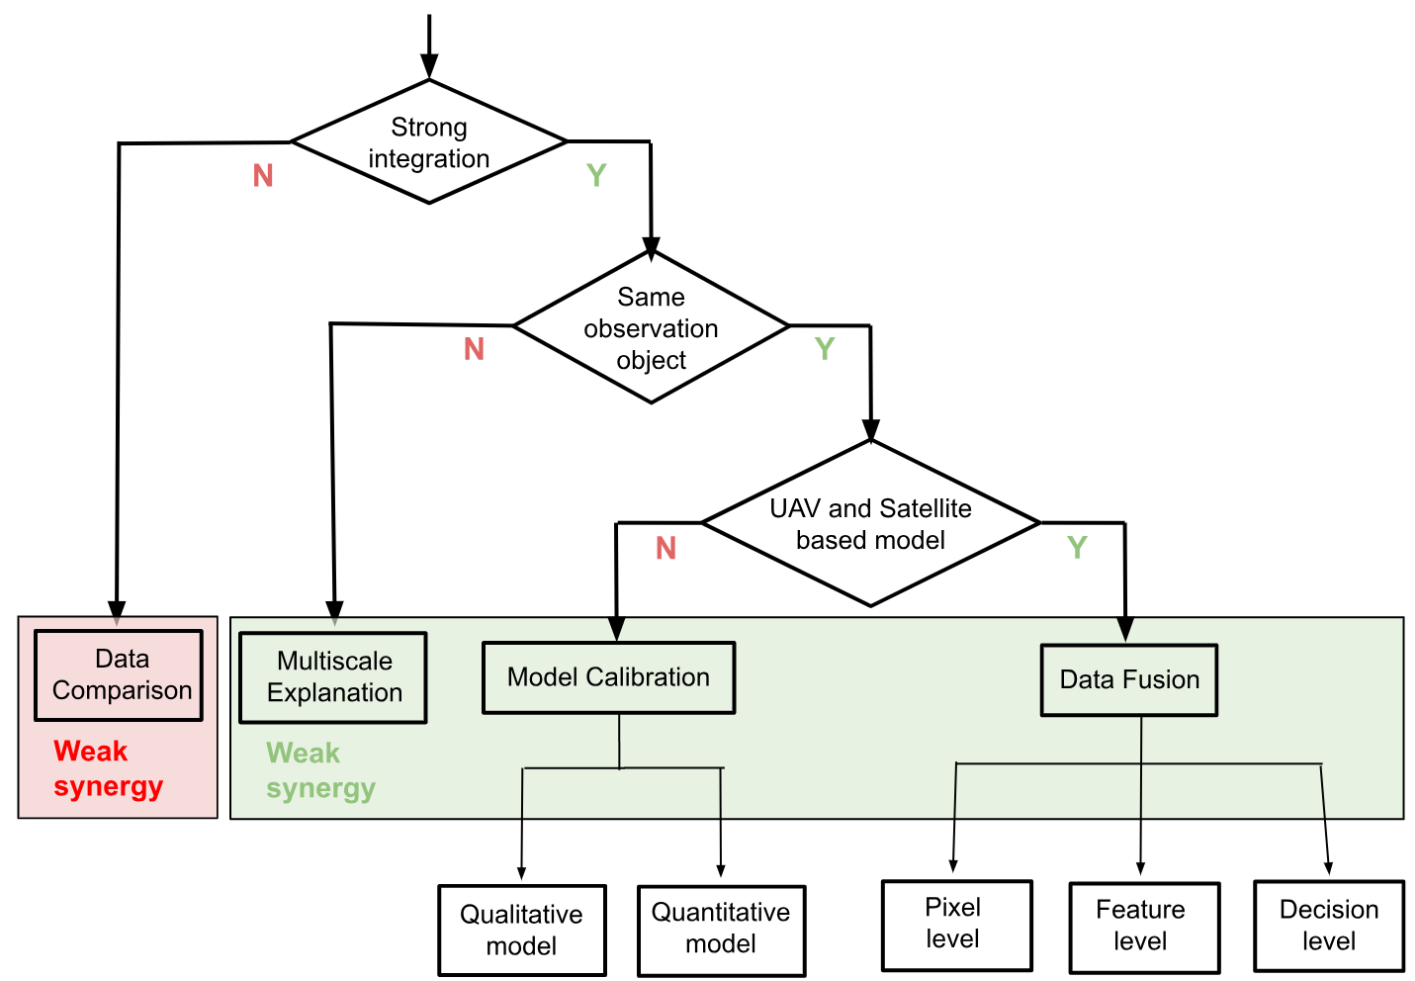
\includegraphics[width=0.8
    \textwidth]{chapters/chapter3/images/Figure11.png}
    \caption{Hierarchical decision tree for categorizing UAV/Satellite strategies \parencite{AlvarezVanhard2021}.}
    \label{fig:UAVSatelliteStrategies}
\end{figure}


\subsubsection{Data comparison strategy}
The data comparison strategy represents a weak form of UAV/Satellite synergy, where data from both sources are analyzed separately rather than combined (Figure~\ref{fig:DataComparison}). These studies highlight the complementary strengths of each platform: satellites offer broad coverage and standardized processing, which is useful for monitoring large or inaccessible areas, while UAVs provide very high spatial resolution (VHSR) at low cost, which is ideal for capturing fine details like crop variability or small water bodies. UAVs are especially valuable in precision agriculture due to their flexibility in capturing data at critical times for input decisions. Ultimately, the choice between UAV and satellite data depends on the study's scale, goals, and available resources. Notably, 19\% of these comparison studies acknowledged the potential for stronger synergies in the future \parencite{AlvarezVanhard2021}.

\begin{figure}[H]
    \centering
    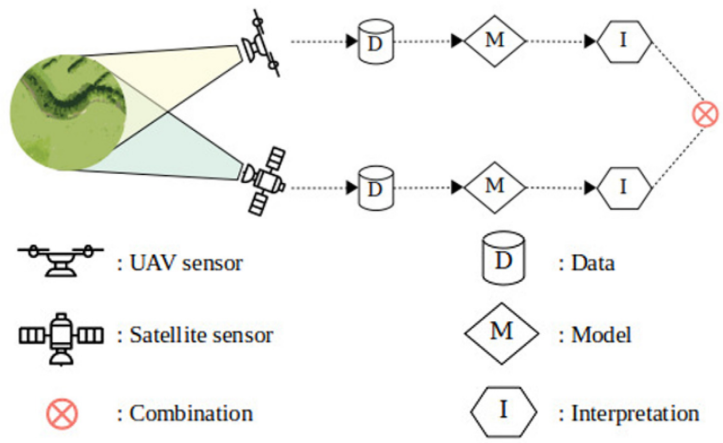
\includegraphics[width=0.6
    \textwidth]{chapters/chapter3/images/Figure12.png}
    \caption{Diagram of data comparison strategy \parencite{AlvarezVanhard2021}.}
    \label{fig:DataComparison}
\end{figure}


\subsubsection{Multiscale explanation strategy}
The multiscale explanation strategy leverages the different spatial scales of UAV and satellite data to enhance interpretation (Figure~\ref{fig:MultiscaleExplanation}). Satellites provide a broad, regional context, while UAVs offer detailed, fine-scale information. This strategy enables better understanding by combining wide-area observation with localized, high-resolution insights, often using UAV-derived digital surface models (DSMs) to refine spatial analysis \parencite{AlvarezVanhard2021}.

\begin{figure}[H]
    \centering
    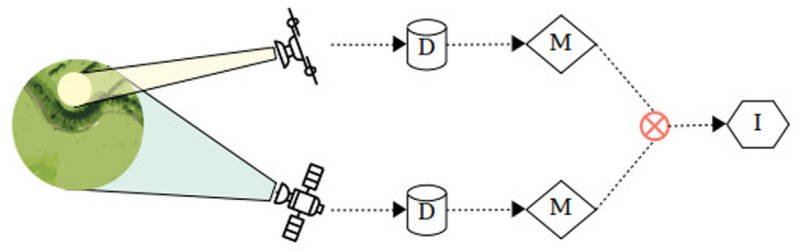
\includegraphics[width=0.6
    \textwidth]{chapters/chapter3/images/Figure13.png}
    \caption{Diagram of the Multiscale explanation strategy \parencite{AlvarezVanhard2021}.}
    \label{fig:MultiscaleExplanation}
\end{figure}

\subsubsection{Model calibration strategy}
The model calibration strategy involves using one data source, often UAV or satellite imagery, to calibrate models built on the other (Figure~\ref{fig:ModelCalibration}). It was the most frequently used strong synergy approach, especially in ecology and precision agriculture. This strategy can be qualitative, where UAV-derived labels (from expert interpretation, thresholds, or classifications) train satellite-based classification models, or quantitative, where UAV-derived numerical values (e.g., chlorophyll, biomass, height) calibrate regression or unmixing models. In some cases, UAV data replaces traditional ground surveys, serving as the sole reference source. While in-situ data is still used in many studies for validation, UAVs are increasingly relied upon for producing accurate, high-resolution ground truth. The strategy also includes data intercalibration, where one dataset is used to standardize or refine the spectral characteristics of the other \parencite{AlvarezVanhard2021}.


\begin{figure}[H]
    \centering
    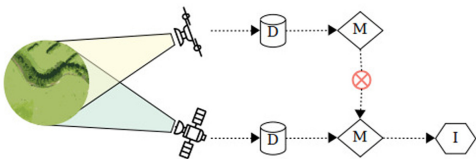
\includegraphics[width=0.6
    \textwidth]{chapters/chapter3/images/Figure14.png}
    \caption{Diagram of Model calibration strategy \parencite{AlvarezVanhard2021}.}
    \label{fig:ModelCalibration}
\end{figure}


\subsubsection{Data fusion strategy}

The data fusion strategy represents the strongest form of UAV/Satellite synergy, aiming to fully integrate both data sources to create enhanced datasets (Figure~\ref{fig:DataFusion}). Though less commonly used, it has been explored in precision agriculture for extracting fine-resolution land cover and vegetation traits. Most studies applied pixel-level fusion to combine spatial, spectral, or temporal details, improving classification accuracy, resolution, or time-series completeness. Some studies used feature-level fusion, integrating complementary views from UAVs and satellites for tasks like damage assessment or change detection. While decision-level fusion holds potential, it has not yet been applied in this context. Overall, data fusion enables more accurate and consistent monitoring by leveraging the unique strengths of both platforms \parencite{AlvarezVanhard2021}.

\begin{figure}[H]
    \centering
    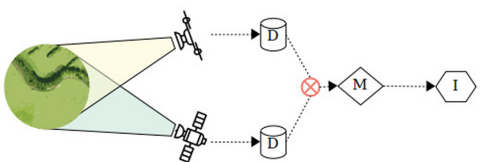
\includegraphics[width=0.6
    \textwidth]{chapters/chapter3/images/Figure15.png}
    \caption{Diagram of Data fusion strategy \parencite{AlvarezVanhard2021}.}
    \label{fig:DataFusion}
\end{figure}

\subsection{Challenges of UAV/Satellite Data Fusion}
While combining UAV and satellite data offers great potential, it also presents several challenges, including:

\begin{itemize}
    \item \textbf{Limited Exploitation of Synergy:} The potential of UAV/Satellite synergy remains underexploited, as most studies prioritize validation or simple comparisons rather than full integration; advanced strategies like multiscale explanation and data fusion, which preserve and leverage the strengths of both data sources, are still rarely applied \parencite{AlvarezVanhard2021}.
  
    \item \textbf{Interoperability Issues:} Interoperability is a major challenge due to the lack of standardization in UAV data acquisition and quality assurance, unlike standardized satellite data; variations in sensors, protocols, and conditions further complicate the alignment of multi-source datasets \parencite{AlvarezVanhard2021}.
  
    \item \textbf{Geometric and Radiometric Misalignment:} Geometric and radiometric misalignment pose a challenge, as misregistration between UAV and satellite data impacts multi-scale analysis; sub-pixel geometric calibration is difficult due to resolution gaps, and radiometric inconsistencies from sensor and environmental differences further hinder seamless integration \parencite{AlvarezVanhard2021}.
  
    \item \textbf{Technical Complexity:} Fusion of UAV and satellite data remains technically complex, as advanced methods like spatio-temporal and spectral-temporal fusion require specialized expertise, making them less accessible and limiting wider adoption \parencite{AlvarezVanhard2021}.
  \end{itemize}
  

\section{Challenges in Integrating Remote Sensing with ML/DL}
Despite the promising results obtained from integrating UAV-based remote sensing with deep learning techniques for crop disease detection, several challenges hinder their widespread and effective adoption in real-world agricultural settings. One of the primary limitations is the scarcity of labeled datasets, which are crucial for training deep learning models. Collecting and annotating high-quality images, especially for specific diseases like wheat rusts, is labor-intensive and often inconsistent across studies \parencite{shahi2023recent}.

Another significant challenge is the high computational complexity associated with training and deploying deep learning models. These models typically require powerful hardware, large memory, and long training times, which can be impractical for use in field conditions or developing regions with limited resources \parencite{shahi2023recent}.

Furthermore, the selection of optimal models remains non-trivial. The performance of deep learning models can vary significantly depending on the type of crop, disease severity, environmental conditions, and sensor data used. This variation complicates the generalization of models across different agricultural scenarios \parencite{shahi2023recent}.

\section{Future Perspectives}
UAV-based plant disease detection is an evolving field with considerable potential for advancement through machine learning (ML) and remote sensing technologies. However, current methods, particularly those involving complex deep learning models like CNNs, can be computationally demanding and require significant resources \parencite{Kouadio2023}. To address these limitations, future research should focus on developing lightweight, edge-compatible models for real-time, on-device analysis, as well as exploring reinforcement learning and sensor fusion (e.g., combining UAV and satellite data) to enhance disease detection accuracy \parencite{shahi2023recent,Kouadio2023}. Reducing dependence on large annotated datasets through semi-supervised learning and establishing benchmark datasets for standardizing model evaluation are also critical steps forward \parencite{shahi2023recent}. Additionally, addressing practical challenges such as the cost of thermal or electrochemical sensors and the technical skill required for drone operation will be essential for widespread adoption, particularly in diverse global agricultural contexts \parencite{Kouadio2023}.

\section{Conclusion}
The integration of remote sensing with machine learning and deep learning has opened new possibilities for the efficient and accurate detection of wheat diseases. By leveraging data from satellites, UAVs, and other sensing platforms, combined with advanced learning algorithms, it is now possible to monitor crop health at scale, detect early signs of infection, and support timely intervention. This chapter highlighted the main technologies, workflows, and challenges involved in this integration, emphasizing its value in enhancing disease management and promoting sustainable agricultural practices. Continued research and refinement of these methods will be essential to fully realize their potential in real-world farming environments.